%% LyX 2.3.6.1 created this file.  For more info, see http://www.lyx.org/.
%% Do not edit unless you really know what you are doing.
\documentclass[11pt,oneside,american,czech]{book}
\usepackage[T1]{fontenc}
\usepackage[utf8]{inputenc}
\usepackage[a4paper]{geometry}
\geometry{verbose,tmargin=4cm,bmargin=3cm,lmargin=3cm,rmargin=2cm,headheight=0.8cm,headsep=1cm,footskip=0.5cm}
\pagestyle{headings}
\setcounter{secnumdepth}{3}
\usepackage{url}
\usepackage{amsmath}
\usepackage{amsthm}
\usepackage{amssymb}
\usepackage{graphicx}
\usepackage{setspace}
\usepackage{listings}
\usepackage[dvipsnames,table,xcdraw]{xcolor}
\usepackage[T1]{fontenc}
\usepackage{lmodern}
\usepackage{pdfpages}
\usepackage{longtable}
\usepackage{multirow}

\definecolor{mygreen}{rgb}{0,0.6,0}
\definecolor{mygray}{rgb}{0.5,0.5,0.5}
\definecolor{mymauve}{rgb}{0.58,0,0.82}
\definecolor{mystring}{rgb}{0.9,0.1,0.2}

\lstset{ 
  backgroundcolor=\color{white},   % choose the background color; you must add \usepackage{color} or \usepackage{xcolor}; should come as last argument
  basicstyle=\scriptsize\fontfamily{cmtt}\selectfont,        % the size of the fonts that are used for the code
  breakatwhitespace=false,         % sets if automatic breaks should only happen at whitespace
  breaklines=true,                 % sets automatic line breaking
  captionpos=t,                    % sets the caption-position to bottom
  commentstyle=\color{mygreen},    % comment style
  stringstyle=\color{mystring},
  deletekeywords={...},            % if you want to delete keywords from the given language
  escapeinside={\%*}{*)},          % if you want to add LaTeX within your code
  extendedchars=true,              % lets you use non-ASCII characters; for 8-bits encodings only, does not work with UTF-8
  firstnumber=1,                   % start line enumeration with line 1000
  frame=single,	                   % adds a frame around the code
  keepspaces=true,                 % keeps spaces in text, useful for keeping indentation of code (possibly needs columns=flexible)
  keywordstyle=\color{blue},       % keyword style
  language=Python,                 % the language of the code
  morekeywords={*,...},            % if you want to add more keywords to the set
  numbers=left,                    % where to put the line-numbers; possible values are (none, left, right)
  numbersep=5pt,                   % how far the line-numbers are from the code
  numberstyle=\tiny\color{mygray}, % the style that is used for the line-numbers
  rulecolor=\color{black},         % if not set, the frame-color may be changed on line-breaks within not-black text (e.g. comments (green here))
  showspaces=false,                % show spaces everywhere adding particular underscores; it overrides 'showstringspaces'
  showstringspaces=false,          % underline spaces within strings only
  showtabs=false,                  % show tabs within strings adding particular underscores
  stepnumber=2,                    % the step between two line-numbers. If it's 1, each line will be numbered
  stringstyle=\color{mymauve},     % string literal style
  tabsize=2,	                   % sets default tabsize to 2 spaces
  title=\lstname                   % show the filename of files included with \lstinputlisting; also try caption instead of title
}

\makeatletter
%%%%%%%%%%%%%%%%%%%%%%%%%%%%%% Textclass specific LaTeX commands.
\newenvironment{lyxlist}[1]
	{\begin{list}{}
		{\settowidth{\labelwidth}{#1}
		 \setlength{\leftmargin}{\labelwidth}
		 \addtolength{\leftmargin}{\labelsep}
		 \renewcommand{\makelabel}[1]{##1\hfil}}}
	{\end{list}}

%%%%%%%%%%%%%%%%%%%%%%%%%%%%%% User specified LaTeX commands.
%% Font setup: please leave the LyX font settings all set to 'default'
%% if you want to use any of these packages:

%% Use Times New Roman font for text and Belleek font for math
%% Please make sure that the 'esint' package is turned off in the
%% 'Math options' page.
\usepackage[varg]{txfonts}

%% Use Utopia text with Fourier-GUTenberg math
%\usepackage{fourier}

%% Bitstream Charter text with Math Design math
%\usepackage[charter]{mathdesign}

%%---------------------------------------------------------------------

%% Make the multiline figure/table captions indent so that the second
%% line "hangs" right below the first one.
%\usepackage[format=hang]{caption}

%% Indent even the first paragraph in each section
\usepackage{indentfirst}

%%---------------------------------------------------------------------

%% Disable page numbers in the TOC. LOF, LOT (TOC automatically
%% adds \thispagestyle{chapter} if not overriden
%\addtocontents{toc}{\protect\thispagestyle{empty}}
%\addtocontents{lof}{\protect\thispagestyle{empty}}
%\addtocontents{lot}{\protect\thispagestyle{empty}}

%% Shifts the top line of the TOC (not the title) 1cm upwards 
%% so that the whole TOC fits on 1 page. Additional page size
%% adjustment is performed at the point where the TOC
%% is inserted.
%\addtocontents{toc}{\protect\vspace{-1cm}}

%%---------------------------------------------------------------------

% completely avoid orphans (first lines of a new paragraph on the bottom of a page)
\clubpenalty=9500

% completely avoid widows (last lines of paragraph on a new page)
\widowpenalty=9500

% disable hyphenation of acronyms
\hyphenation{CDFA HARDI HiPPIES IKEM InterTrack MEGIDDO MIMD MPFA DICOM ASCLEPIOS MedInria}

%%---------------------------------------------------------------------

%% Print out all vectors in bold type instead of printing an arrow above them
\renewcommand{\vec}[1]{\boldsymbol{#1}}

% Replace standard \cite by the parenthetical variant \citep
%\renewcommand{\cite}{\citep}

\makeatother

\usepackage{babel}
\begin{document}
\def\documentdate{10. května 2024}

%%\def\documentdate{\today}

\pagestyle{empty}
{\centering

\noindent %
\begin{minipage}[c]{3cm}%
\noindent \begin{center}

\includegraphics[width=3cm,height=3cm,keepaspectratio]{Images/TITLE/cvut}
\par\end{center}%
\end{minipage}%
\begin{minipage}[c]{0.6\linewidth}%
\begin{center}
\textsc{\large{}České vysoké učení technické v Praze}{\large{}}\\
{\large{}Fakulta jaderná a fyzikálně inženýrská}
\par\end{center}%
\end{minipage}%
\begin{minipage}[c]{3cm}%
\noindent \begin{center}

\includegraphics[width=3cm,height=3cm,keepaspectratio]{Images/TITLE/fjfi}
\par\end{center}%
\end{minipage}

\vspace{3cm}

\textbf{\huge{}Moderní metody robustního strojového učení}{\huge\par}

\vspace{1cm}

\selectlanguage{american}%
\textbf{\huge{}Modern methods of robust machine learning}{\huge\par}

\selectlanguage{czech}%
\vspace{2cm}

{\large{}Diplomová práce}{\large\par}

}

\vfill{}

\begin{lyxlist}{MMMMMMMMM}
\begin{singlespace}
\item [{Autor:}] \textbf{Bc. Pavel Jakš}
\item [{Vedoucí~práce:}] \textbf{Mgr. Lukáš Adam, Ph.D.}
\item [{Konzultant:}] \textbf{Ing. Pavel Strachota, Ph.D.}
\item [{Akademický~rok:}] 2023/2024
\end{singlespace}
\end{lyxlist}
\newpage{}

\includepdf{zadani_dp.pdf}

\includepdf[page=2]{zadani_dp.pdf}

\newpage{}

\noindent \emph{\Large{}Poděkování:}{\Large\par}

\noindent Chtěl bych zde poděkovat především svému školiteli panu doktoru Adamovi
za pečlivost, ochotu, vstřícnost a odborné i lidské zázemí při vedení
mé diplomové práce. Dále děkuji svému konzultantovi panu doktoru Strachotovi
za jeho odborné rady.

\vfill

\noindent \emph{\Large{}Čestné prohlášení:}{\Large\par}

\noindent Prohlašuji, že jsem tuto práci vypracoval samostatně a uvedl
jsem všechnu použitou literaturu.

\bigskip{}

\noindent V Praze dne 10. května 2024\hfill{}Bc. Pavel Jakš

\vspace{2cm}

\newpage{}

\begin{onehalfspace}
\noindent \emph{Název práce:}

\noindent \textbf{Moderní metody robustního strojového učení}
\end{onehalfspace}

\bigskip{}

\noindent \emph{Autor:} Bc. Pavel Jakš

\bigskip{}

\noindent \emph{Obor:} Matematická informatika\bigskip{}

\bigskip{}

\noindent \emph{Druh práce:} Diplomová práce

\bigskip{}

\noindent \emph{Vedoucí práce:} Mgr. Lukáš Adam, Ph.D.,
Katedra počítačů,
Fakulta elektrotechnická,
České vysoké učení technické v Praze,
Karlovo náměstí 13, 121 35 Praha 2.

\bigskip{}

\noindent \emph{Konzultant:} Ing. Pavel Strachota, Ph.D.,
Katedra matematiky,
Fakulta jaderná a fyzikálně inženýrská,
České vysoké učení technické v Praze,
Trojanova 13, 120 00 Praha 2.

\bigskip{}

\noindent \emph{Abstrakt:}
V oblasti strojového učení se vyskytl problém existence tak zvaných adversariálních vzorků.
Jedná se o jev, kdy i malá změna vstupu nějakého modelu strojového učení
způsobí velikou změnu výstupu, což je ve většině případech nežádoucí.
V této práci se potom věnujeme problematice metrik vizuální podobnosti,
a to právě v kontextu existence a tvorby adversariálnich vzorků v oblasti klasifikace obrázků.
Naším cílem je osvětlit, jakým způsobem taková metrika vizuální podobnosti ovlivní
proces tvorby adversariálních vzorků a jejich podobu.

\bigskip{}

\noindent \emph{Klíčová slova:}
Adversariální vzorky,
CW útok,
Foolbox,
$l_p$ norma,
metrika vizuální podobnosti,
neuronová síť,
PSNR,
robustní strojové učení,
RobustBench,
SSIM,
Wassersteinova metrika.

\vfill{}
~

\selectlanguage{american}%
\begin{onehalfspace}
\noindent \emph{Title:}

\noindent \textbf{Modern methods of robust machine learning}
\end{onehalfspace}

\bigskip{}

\noindent \emph{Author:} Bc. Pavel Jakš

\bigskip{}

\noindent \emph{Abstract:}
There exists a problem in the field of machine learning called adversarial examples.
This is a phenomenon where even a small change of the input to a machine learning model
causes a big difference in the model output, which is in most cases unwanted.
In this work we study the questions concerning visual similarity metrics
and that in the context of existence and crafting of adversarial examples in the problem of image classification.
Our goal is to enlighten hte way how such a visual similarity metric affects
the crafting process of adversarial examples and their final look.

\bigskip{}

\noindent \emph{Key words:}
Adversarial examples,
CW attack,
Foolbox,
$l_p$ norm,
neural network,
PSNR,
robust machine learning,
RobustBench,
SSIM,
visual similarity metric,
Wasserstein metric.

\selectlanguage{czech}%
\newpage{}

\pagestyle{plain}

\tableofcontents{}

\newpage{}

\chapter*{Úvod}

\addcontentsline{toc}{chapter}{Úvod}

V této práci se věnujeme problematice metrik vizuální podobnosti,
a to v kontextu strojového učení,
konrétně v oblasti existence a tvorby adversariálnich vzorků.
Zkoumáme, jaký vliv má volba takové metriky na tvorbu a podobu adversariálních vzorků.

V první kapitole představujeme samotné metriky vizuální podobnosti.
Jelikož obrázky v počítači, s nimiž pracujeme, lze chápat jako tenzory,
lze se podívat na obrázky v klasické $l_p$ normě.
Část této kapitoly se proto věnuje formální definici těchto $l_p$ norem
a toho, jak z nich zkonstuovat metriku.
Zmiňujeme i metriky založené na průměrování rozdílů prvků vektorů,
tedy metriky MSE (\emph{mean squared error}) a RMSE (\emph{root mean squared error}),
dále i jejich logaritmickou transformaci známou pod zkratkou PSNR (\emph{peak signal to noise ratio}).
Další konstrukce, které představujeme jsou SSIM, tedy \emph{Structural Similarity Index Measure},
a \emph{Wassersteinova metrika}, která se na obrázky dívá jako na pravděpodobnostní rozdělení.

V druhé kapitole pak narážímme na výpočetní limity a fakt, že ne všechny metriky vizuální podobnosti
jsou metriky podle matematické definice.
Proto uvedeme alternativu k PSNR, transformaci SSIM a regularizaci Wassersteinovy metriky,
které pomohou překonat tyto problémy pro praktickou tvorbu adversariálních vzorků.

Třetí kapitola potom pojednává o samotné problematice adversariálních vzorků,
o jejich definici a o jednom z mnoha přístupů k jejich praktické tvorbě.
Nastiňujeme také rozdíl mezi \emph{cíleným} (angl. \emph{targeted}) a \emph{necíleným} (angl. \emph{untargeted})
adversariálním útokem.

Ve čtvrté kapitole pak uvádíme samotné výsledky použití vybraných metrik vizuální podobnosti
pro tvorbu adversariálních vzorků pomocí necíleného \emph{CW} útoku.
Porovnáváme, jak procentuální úspěšnost útoku v dané metrice,
tak průměrnou $l_2$ vzdálenost výsledků procedury s původními vzorky.

Poslední pátá kapitola pak nastiňuje problematiku robustního strojového učení,
tedy disciplíny, která se snaží existenci adversariálních vzorků zabránit
vhodnými metodami pro daný algoritmus strojového učení.
Uvádíme také, jak se jakousi robustnost obzvlášť neuronových sítí vůči adversariálním útokům
snaží měřit programovací knihovny \emph{Foolbox} a \emph{RobustBench}.

\pagestyle{headings}

\chapter{Metriky vizuální podobnosti}

Metrika vizuální podobnosti je nástroj, který umožňuje, jak napovídá sám název,
měřit, jak jsou si dva vizuální vjemy podobné.
Pod vizuálním jevem zde v kontextu strojového učení myslíme strojově
zpracovatelný vizuální vjem, tedy obrázek.
Tedy obecně se jedná o tenzor z množiny $\mathbb{M}^{C \times W \times H}$,
kde $\mathbb{M}$ je podmnožina reálných čísel, za kterou volíme například množinu $\{0, 1, ..., 255\}$,
tedy diskrétní hodnoty pizelů, které lze reprezentovat pomocí $8$ bitů,
nebo třeba za $\mathbb{M}$ volíme  interval $[0, 1]$.
Parametry $C$, $W$, $H$ potom reprezentují po řadě počet kanálů obrázku,
šířku obrázku a výšku obrázku.
V praxi se nejčastěji setkáme se šedotónovými obrázky, potom $C = 1$,
nebo s obrázky typu \emph{RGB}, kde $C = 3$ a jednotlivé kanály reprezentují po řadě červenou, zelenou a modrou barvu.
Alternativní přístup k obrázku je potom reprezentace pomocí tenzorů $\mathbb{M}^{W \times H \times C}$,
kdy měníme pořadí indexace jednotlivých prvků tenzoru.
V této práci potom užíváme první z konvencí.
Důvodem je, že tato konvence je vlastní knihovně \emph{PyTorch}, která je zde užita.
Máme tedy ujasněno slovo \emph{vizuální} z termínu \emph{metriky vizuální podobnosti}.

Pod pojmem \emph{podobnost} si potom představme to, jaké společné rysy dva takové obrázky mají.
Může se jednat o vyobrazení stejného objektu či o informaci, kterou nesou.
Nebo prostě blízkost ve smyslu pohledu na obrázky jako na dva tenzory.

Nakonec rozveďme pojem metrika.
Slovo metrika v první řadě vyjadřuje propojení vzdálenosti nebo podobnosti
ve výše uvedeném smyslu s jedním konkrétním reálným číslem.
Metrika je tedy zobrazení, které na vstupu bere dva prvky stejné množiny a vrací číslo,
které vyjadřuje, jak moc si jsou tyto dva objekty blízko či jak jsou si tyto dva objekty podobné.
Metriku lze ovšem formálně matematicky definovat, aby dávala v konečném důsledku vzniknout topologii,
což je nástroj, kterým vybavíme-li libovolnou množinu, můžeme nakládat s pojmy jako je okolí bodu,
otevřená množina či kompaktnost.
Pod pojmem metrika na prostoru $X$ si tedy každý matematik představí zobrazení $\rho : X \times X \rightarrow [0, + \infty)$
splňující
\begin{enumerate}
    \item $\rho(x, y) = 0 \iff x = y \quad \forall x, y \in X$,
    \item $\rho(x, y) = \rho(y, x) \quad \forall x, y \in X$,
    \item $\rho(x, z) \leq \rho(x, y) + \rho(y, z) \quad \forall x, y, z \in X$.
\end{enumerate}

Taková metrika může být na lineárním prostoru $V$ nad číselným tělesem (pro naše účely zůstaňme nad $\mathbb{R}$)
snadno zadána pomocí normy,
která je buď indukována skalárním součinem v případě pre-Hilbertových prostorů,
nebo dána vlastnostmi, že se jedná o zobrazení $\|.\| : V \rightarrow [0, + \infty)$
a splňuje:
\begin{enumerate}
    \item $\|x\| = 0 \iff x = 0 \quad \forall x \in V$,
    \item $\|\alpha x\| = |\alpha| \cdot \|x\| \quad \forall \alpha \in \mathbb{R}, \forall x \in V$,
    \item $\|x + y\| \leq \|x\| + \|y\| \quad \forall x, y \in V$.
\end{enumerate}
Metriku potom získáme z normy následující konstrukcí:
\begin{equation*}
    \rho (x, y) = \| x - y \|,
\end{equation*}
tedy vzdálenost dvou vektorů je dána normou rozdílu vektorů.
Snadno lze nahlédnout, že takto zadané zobrazení je metrika.
S metrikami, které jsou tzv. indukované normami dle předchozího se setkáme.


\section{Metriky indukované $l_p$ normami}

Vzhledem k tomu, že obrázky, které jsou středem naší pozornosti,
lze reprezentovat jako tenzory o rozměrech $C \times W \times H$,
kde $C$, $W$ a $H$ jsou jako výše, tak lze tyto tenzory použít jako vstup pro $L^p$ normy.
Pro $p \in [1, + \infty)$ je $L^p$ norma z $f \in L_p(X, \mu )$
definována vztahem:
\begin{equation*}
    \|f\|_p = \left(\int_X |f|^p \mathrm{d} \mu \right)^{\frac{1}{p}}.
\end{equation*}

Pro naše obrázky lze za $X$ vzít $\{1, ... C\} \times \{1, ..., W\} \times \{1, ..., H\}$ a za $\mu$ \emph{počítací míru}.
Potom naše $L^p$ norma přejde v $l_p$ normu, která má pro naše obrázky, tedy tenzory $x \in \mathbb{R}^{C \times W \times H}$, tvar:
\begin{equation}
    \|x\|_p = \left( \sum_{i=1}^{C} \sum_{j=1}^{W} \sum_{k=1}^{H} |x_{i, j, k}|^p \right)^{\frac{1}{p}}.
\end{equation}

Této definici se potom vymyká $l_{\infty}$ norma, která má tvar pro tenzor $x \in \mathbb{R}^{C \times W \times H}$:
\begin{equation}
    \|x\|_\infty = \max_{i \in \{1, ..., C\}} \max_{j \in \{1, ..., W\}} \max_{k \in \{1, ..., H\}} |x_{i, j, k}|.
\end{equation}

% A úplně mimo stojí $L_0$ norma, která svou povahou \emph{není} norma ve smyslu výše uvedené definice,
% ale pro účely porovnávání obrázků se používá rozdíl obrázků v této pseudo-normě, proto ji zde zmiňuji:
% \begin{equation}
%     \|x\|_0 = |\{x_{i, j, k} \neq 0\}|.
% \end{equation}

\section{MSE a RMSE}

Vzdálenosti, které mají blízko k metrikám indukovaným $l_2$ normou, jsou \emph{MSE} (z anglického \emph{Mean Squared Error})
a \emph{RMSE} (z anglického \emph{Root Mean Squared Error}).
Pro tenzory $x, \tilde{x} \in \mathbb{R}^{C \times W \times H}$ mají definici:
\begin{align}
    \operatorname{MSE}(x, \tilde{x}) &= \frac{1}{C W H} \sum_{i=1}^C \sum_{j=1}^W \sum_{k=1}^H | x_{i, j, k} - \tilde{x}_{i, j, k} |^2 \\
    \operatorname{RMSE}(x, \tilde{x}) &= \left(\frac{1}{C W H} \sum_{i=1}^C \sum_{j=1}^W \sum_{k=1}^H | x_{i, j, k} - \tilde{x}_{i, j, k} |^2 \right)^{\frac{1}{2}}
\end{align}
Jedná se vlastně o transformaci metriky založené na $l_2$ normě.
Platí totiž:
\begin{align}
    \operatorname{MSE}(x, \tilde{x}) = \frac{1}{CWH} \|x - \tilde{x}\|_2^2 \\
    \operatorname{RMSE}(x, \tilde{x}) = \frac{1}{\sqrt{CWH}} \|x - \tilde{x}\|_2 
\end{align}
Tyto metriky vizuální podobnosti potom sehrávají roli,
chceme-li porovnávat rozdíly mezi obrázky napříč obrázky různých rozměrů.
Samozřejmě to ale neznamená, že získáme vzdálenost dvou obrázků, které mají každý jiný rozměr.

\section{Peak signal-to-noise ratio}

Vzdálenost označená zkratkou \emph{PSNR} z anglického \emph{peak signal-to-noise ratio}
vyjadřuje vztah mezi obrázkem $x \in \mathbb{R}^{C \times W \times H}$
a jeho pokažením $\tilde{x} \in \mathbb{R}^{C \times W \times H}$,
což je obrázek, který má zásadě nést stejnou informaci, ale je poškozený,
a to ať už rozmazáním nebo šumem.
Cílem této metriky vizuální podobnosti je potom kvantitativně vyjádřit právě míru šumu.
Definice je následující:
\begin{align} \label{PSNR_def}
    \operatorname{PSNR}(x, \tilde{x}) &= 10 \cdot \operatorname{log}_{10} \left( \frac{l^2}{\operatorname{MSE}(x, \tilde{x})} \right), \\
    &= 20 \cdot \operatorname{log}_{10} \left( \frac{l}{\operatorname{RMSE}(x, \tilde{x})} \right),
\end{align}
kde $l$ je dynamický rozsah obrázků, tedy rozdíl mezi maximální možnou hodnotou pixelů a minimální možnou hodnotou pixelů.
% Jak je vidět, prohození $x$ a $\tilde{x}$ povede ke změně hodnoty $\operatorname{PSNR}$, tato vzdálenost tedy není metrická.
Jedná se tedy o transformaci metriky \emph{MSE}.
Samotná hodnota PSNR ovšem není metrická vzdálenost.
Vždyť budou-li se obrázky $x$ a $\tilde{x}$ blížit k sobě, hodnota $\operatorname{PSNR}(x, \tilde{x})$ poroste do nekonečna,
neboť jmenovatel argumentu v logaritmu v definici (\ref{PSNR_def}) jde k nule, a to zprava,
tudíž argument logaritmu jde do $+\infty$ a tedy i logaritmus roste do $+\infty$.
Toto odpovídá tomu, že šum v pokažení $\tilde{x}$ je nulový.

\section{Wassersteinova vzdálenost}

Buď $(M, \rho)$ metrický prostor. Zvolme $p \in [1, + \infty)$.
Potom máme \emph{Wassersteinovu $p$-vzdálenost} mezi dvěma pravděpodobnostními mírami $\mu$ a $\nu$ na $M$,
které mají konečné $p$-té momenty,
jako:
\begin{equation} \label{wass_def}
    W_p (\mu, \nu) = \left( \inf_{\gamma \in \Gamma(\mu, \nu)} \mathbb{E}_{(x, y) \sim \gamma} \rho (x, y)^p \right)^{\frac{1}{p}},
\end{equation}
kde $\Gamma(\mu, \nu)$ je množina všech sdružených pravděpodobnostních měr na $M \times M$,
které mají po řadě $\mu$ a $\nu$ za marginální pravděpodobnostní míry \cite{vaserstejn}.

Jak to souvisí s obrázky?
Přes dopravní problém.
Pod pravděpodobnostní distribucí $\mu$ či $\nu$ na $X$ si lze představit rozložení jakési hmoty
o celkové hmotnosti $1$.
Sdružená rozdělení $\gamma \in \Gamma(\mu, \nu)$ potom odpovídají transportnímu plánu,
kde $\gamma(x, y) \, dx \, dy$
vyjadřuje, kolik hmoty se přesune z $x$ do $y$.
Tomu lze přiřadit nějakou cenu $c$,
totiž kolik stojí přesun jednotkové hmoty z $x$ do $y$: $c(x, y)$.
V případě \emph{Wassersteinovy vzdálenosti}
za cenu dosadíme $c(x, y) = \rho(x, y)^p$,
tedy $p$-tou mocninu vzdálenosti mezi $x$ a $y$.
Potom cena celkového dopravního problému s transportním plánem $\gamma$ bude:
\begin{equation}
    c_\gamma = \int c(x, y) \gamma(x, y) \, dx \, dy
\end{equation}
a optimální cena bude:
\begin{equation}
    c = \inf_{\gamma \in \Gamma(\mu, \nu)} c_\gamma.
\end{equation}
Po dosazení:
\begin{align}
    c &= \inf_{\gamma \in \Gamma(\mu, \nu)} \int c(x, y) \gamma(x, y) \, dx \, dy \\
    &= \inf_{\gamma \in \Gamma(\mu, \nu)} \mathbb{E}_{(x, y) \sim \gamma} c(x, y) \\
    &= \inf_{\gamma \in \Gamma(\mu, \nu)} \mathbb{E}_{(x, y) \sim \gamma} \rho(x, y)^p \\
    &= W_p (\mu, \nu)^p
\end{align}
Dostáváme tedy interpretaci, že $p$-tá mocnina \emph{Wassersteinovy vzdálenosti}
odpovídá ceně dopravního problému.

Pro obrázky má tato konstrukce následující uplatnění:
Obrázky je třeba chápat jako diskrétní pravděpodobnostní rozdělení,
proto je třeba je normalizovat,
aby součet prvků tenzoru obrázku byl roven $1$.
Pak střední hodnota v definici Wassersteinovy vzdálenosti přejde ve váženou sumu cen,
tedy $p$-tých mocnin vzdáleností mezi jednotlivými pixely.

Jak je to barevnými obrázky, tedy s obrázku, které mají více než jeden kanál?
Zde lze uplatnit následující dva přístupy:
\begin{enumerate}
    \item Normovat celý obrázek na jedničku, tedy všechny kanály dohromady, a tím pádem i definovat vzdálenost mezi jednotlivými kanály,
    \item Normovat každý kanál zvlášť na jedničku, počítat Wassersteinovu metriku pro každý kanál zvlášť
    a následně vybrat nějakou statistiku výsledných vzdáleností, např. průměr.
\end{enumerate}

\section{Structural similarity index measure}

Zkratka \emph{SSIM} pochází z anglického \emph{structural similarity index measure}.
Tato metrika se při výpočtu indexu dvou obrázků $x$ a $\tilde{x}$ dívá na podokna,
ze kterých vybere jisté statistiky a z nich vytvoří index pro daná podokna obrázků.
Potom se jako celkový index bere průměr přes tato okna.
Uveďme vzorce pro výpočet indexu SSIM pro případ, že máme jediné okno, které splývá s obrázkem,
které pro jednoduchost zvolme jednokanálové, tedy černobílé.
Označme $N = W \times H$ počet pixelů v obrázku a indexujme prvky matice obrázku jediným číslem.
Potom definujeme pro obrázky $x$ a $\tilde{x}$ následující:
\begin{align*}
    \mu_x &= \frac{1}{N} \sum_{i = 1}^N x_i, \\
    \mu_{\tilde{x}} &= \frac{1}{N} \sum_{i = 1}^N \tilde{x}_i, \\
    \sigma_x^2 &= \frac{1}{N - 1} \sum_{i = 1}^N (x_i - \mu_x)^2, \\
    \sigma_{\tilde{x}}^2 &= \frac{1}{N - 1} \sum_{i = 1}^N (\tilde{x}_i - \mu_{\tilde{x}})^2, \\
    \sigma_{x \tilde{x}} &= \frac{1}{N - 1} \sum_{i = 1}^N (x_i - \mu_x)(\tilde{x}_i - \mu_{\tilde{x}}).
\end{align*}
Tedy proměnné $\mu_x$ a $\mu_{\tilde{x}}$ odpovídají průměru,
$\sigma_x^2$ a $\sigma_{\tilde{x}}^2$ rozptylu
a $\sigma_{x \tilde{x}}$ kovarianci.
Potom definujeme:
% Pod zkratkou \emph{SSIM} (\emph{Structural Similarity Index Measure})
% se rozumí následující vzdálenost:
\begin{equation}
    \operatorname{SSIM}(x, \tilde{x}) = \frac{(2 \mu_x \mu_{\tilde{x}} + C_1)(2 \sigma_{x \tilde{x}} + C_2)}{(\mu_x^2 + \mu_{\tilde{x}}^2 + C_1)(\sigma_x^2 + \sigma_{\tilde{x}}^2 + C_2)},
\end{equation}
% kde $\mu$ je průměr hodnot pixelů $x$, resp. $\tilde{x}$,
% $\sigma_{x \tilde{x}}$ je nestranný odhad kovariance mezi $x$ a $\tilde{x}$,
% $\sigma^2$ je nestranný odhad rozptylu $x$, resp. $\tilde{x}$
kde $C_1, C_2$ jsou konstanty pro stabilitu dělení volené kvadraticky úměrně dynamickému rozsahu.
% Máme-li dva obrázky, tak za $x$ a $\tilde{x}$ do vzorce pro $\operatorname{SSIM}$ se standardně volí jakási okna obrázků.
% To znamená, že za celkovou vzdálenost mezi dvěma obrázky volíme průměr přes všechna okna předem zvolené velikosti.
Tato výsledná statistika je potom součinem tří metrik,
které jsou definovány jako metrika jasu
\begin{equation}
    l(x, \tilde{x}) = \frac{2 \mu_x \mu_{\tilde{x}} + C^{(1)}}{\mu_x^2 + \mu_{\tilde{x}}^2 + C^{(1)}},
\end{equation}
metrika kontrastu
\begin{equation}
    c(x, \tilde{x}) = \frac{2 \sigma_x \sigma_{\tilde{x}} + C^{(2)}}{\sigma_x^2 + \sigma_{\tilde{x}}^2 + C^{(2)}},
\end{equation}
a metrika struktury
\begin{equation}
    s(x, \tilde{x}) = \frac{\sigma_{x \tilde{x}} + C^{(3)}}{\sigma_x \sigma_{\tilde{x}} + C^{(3)}}.
\end{equation}
Volba konstant je potom
\begin{align}
    C^{(1)} &= C_1, \\
    C^{(2)} &= C_2, \\
    C^{(3)} &= \frac{C_2}{2}.
\end{align}
SSIM je pak metrikou vizuální podobnosti kombinující informaci o podobnosti jasu, kontrastu a struktury.
Můžeme si povšimnout, že $\operatorname{SSIM}(x, \tilde{x})$ není metrická vzdálenost.
Budou-li obrázky stejné, nevyjde $0$, nýbrž $1$ \cite{ssim}.
Může se také stát, že SSIM vrátí zápornou hodnotu, která může vzniknout členem $\sigma_{x \tilde{x}}$.
Jak volíme celkový SSIM pro barevné obrázky?
Jako průměr přes kanály.



\chapter{Implementace metrik vizuální podobnosti}

V minulé kapitole jsme viděli přehled metod, jak přistoupit k porovnávání dvou různých obrázků.
Předvedli jsme, jak vyčíslit rozdíl mezi dvěma obrázky.
Ne vždy se ovšem jedná o metriku ve smyslu matematickém,
což pro tvorbu adversariálních vzorků je záhodno,
a ne vždy lze takovouto vzdálenost přímočaře spočíst.
Proto uveďme, je-li to nutné, příslušné úkroky stranou, které nám umožní hledat adversariální vzorky,
a to pokud možno v krátkém čase.

Poznatky z této kapitoly nám potom pomáhají k vlastní implementaci metrik vizuální podobnosti
v programovacím jazyce \emph{Python} \cite{python} za použití knihovny \emph{PyTorch} \cite{pytorch}.

\section{Metriky založené na $l_p$ normách}

Implementovat klasické $l_p$ normy je snadné, a tedy i metriky jimi indukované.
MSE a RMSE jsou též snadné na implementaci.
Vlastně i PSNR.
Metriku vizuální podobnosti PSNR je třeba ovšem ošetřit,
neboť, jak již bylo poznamenáno,
budou-li se obrázky $x$ a $\tilde{x}$ blížit k sobě,
hodnota $\operatorname{PSNR}(x, \tilde{x})$ poroste do nekonečna.
Proto zkusme vzít konstrukci, kde prohodíme roli dynamického rozsahu $l$ (peak signal) s rolí šumu (noise),
dostaneme tedy, co lze nazvat noise to peak signal ratio (NPSR):
\begin{align}
    \operatorname{NPSR}(x, \tilde{x}) &= 20 \cdot \operatorname{log}_{10} \left( \frac{\operatorname{RMSE}(x, \tilde{x})}{l} \right), \\
    &= - \operatorname{PSNR}(x, \tilde{x}).
\end{align}
Při dvou obrázcích blížících se k sobě bude tedy NPSR klesat, a to neomezeně.


\section{Modifikace Wassersteinovy vzdálenosti}

Abychom mohli s Wassersteinovou metrikou nakládat například v počítači, je nutné tuto metriku spočíst.
Podíváme-li se do definice (\ref{wass_def}), znamená to vyřešit optimalizační problém.
Byť bychom se omezili hledání vzdáleností dvou vektorů o~rozměru $q$,
měli bychom problém s časovou složitostí nejlépe $\mathcal{O}(q^3 \operatorname{log} q)$ \cite{wass_computation}.
Bohužel takovou výpočetní kapacitou, která by toto zvládla rychle pro námi používané obrázky nemáme k dispozici.
Proto se podívejme, jak Wassersteinovu vzdálenost spočíst rychleji, byť za cenu ztráty přesnosti.

V následujících odstavcích textu uvažujme, že chceme spočítat vzdálenost mezi diskrétními rozděleními,
jejichž pravděpodobnostními vektory jsou $\mu \in \mathbb{R}^q$ a $\nu \in \mathbb{R}^q$, kde $q \in \mathbb{N}$.
Dále označme $1_q$ vektor, jehož hodnoty v každé souřadnici jsou rovny $1$ a má dimenzi udanou v indexu.
Platí tedy $\mu^T 1_q = \nu^T 1_q = 1$ a $\forall i \; \nu_i \geq 0$ a $\forall j \; \nu_j \geq 0$.
Označme jako $U(\mu, \nu)$ množinu všech matic $P \in \mathbb{R}^{q \times q}, P_{i,j} \geq 0$
takových, že $P 1_q = \nu$ a $P^T 1_q = \mu$.
Jako matici $C$ označme zadanou matici cen, která splňuje, že reprezentuje metriku.
To znamená, že $C_{i, j} \geq 0$, $C_{i, j} = 0 \iff i = j$, $C_{i, j} = C_{j, i}$ a $C_{i, k} \leq C_{i, j} + C_{j, k}$.
Tedy prvek matice $C_{i, j}$ určuje metrickou vzdálenost mezi prvkem $i$ a prvkem $j$.
Potom lze napsat:
\begin{equation}
    W (\mu, \nu) \equiv W_1 (\mu, \nu) = \min_{P \in U(\mu, \nu)} \langle P, C \rangle,
\end{equation}
kde $\langle P, C \rangle = \sum_{i, j = 1}^q P_{i, j} C_{i, j}$.
Toto je důsledkem volby $p = 1$.
To že infimum v definici (\ref{wass_def}) přechází v maimum je dáno tím,
že $U(\mu, \nu)$ je kompaktní podmnožina $\mathbb{R}^{q \times q}$.


\subsection{Sinkhornova metrika}

Začněme s mírnou úpravou původního optimalizačního problému definujícího Wassersteinovu vzdálenost:
Pro $\alpha > 0$ definujme jakési $\alpha$ okolí rozdělení $\mu \nu^T$
(sdružené pravděpodobnostní rozdělení s marginálními $\mu$ a $\nu$, ve kterém $\mu$ a $\nu$ jsou nezávislá rozdělení) ve smyslu
\emph{Kullback-Leiblerovy divergence}
\begin{equation}
    U_{\alpha} (\mu, \nu) = \{P \in U(\mu, \nu) | KL(P \| \mu \nu^T) \leq \alpha\}.
\end{equation}
Připomeňme definici Kullback-Leiblerovy divergence:
\begin{equation*}
    KL(\tilde{P} \| \hat{P}) = \sum_{i = 1}^q \sum_{j = 1}^q \tilde{P}_{i, j} \operatorname{log} \frac{\tilde{P}_{i, j}}{ \hat{P}_{i, j}}.
\end{equation*}
Pro dané $P \in U(\mu, \nu)$ lze na kvantitu $KL(P \| \mu \nu^T)$ nahlédnout jako na informaci mezi veličinami s rozděleními $\mu$ a $\nu$.
Tedy $U_\alpha (\mu, \nu)$ vybírá ta rozdělení, která nesou malou vzájemnou informaci mezi $\mu$ a $\nu$ (ve smyslu menší než $\alpha$).
Potom lze definovat Sinkhornovu metriku:
\begin{equation}
    W^\alpha (\mu, \nu) = \min_{P \in U_\alpha (\mu, \nu)} \langle P, C \rangle.
\end{equation}
Dále na výraz $KL(P \| \mu \nu^T)$ lze nahlédnout následovně:
\begin{align*}
    KL(P \| \mu \nu^T) &= \sum_{i = 1}^q \sum_{j = 1}^q P_{i, j} \operatorname{log} \frac{P_{i, j}}{ \mu_i \nu_j}, \\
    &= \sum_{i = 1}^q \sum_{j = 1}^q P_{i, j} \operatorname{log} P_{i, j} -  \sum_{i = 1}^q \sum_{j = 1}^q P_{i, j} \operatorname{log} \mu_i - \sum_{i = 1}^q \sum_{j = 1}^q P_{i, j} \operatorname{log} \nu_j, \\
    &= \sum_{i = 1}^q \sum_{j = 1}^q P_{i, j} \operatorname{log} P_{i, j} -  \sum_{i = 1}^q \mu_i \operatorname{log} \mu_i - \sum_{j = 1}^q \nu_j \operatorname{log} \nu_j, \\
    &= - H(P) + H(\mu) + H(\nu),
\end{align*}
kde $H$ značí entropii.
Odtud můžeme vidět, že podmínka $KL(P \| \mu \nu^T) \leq \alpha$ znamená, že požadujeme po sdruženém rozdělení $P$,
aby mělo velkou entropii.


\subsection{Duální Sinkhornova metrika}

% Omezme se na prostory konečné dimenze. Potom mějme za úkol spočíst Wassersteinovu  (zvolme $p = 1$)
% vzdálenost vektorů s nezápornými prvky
% $\mu, \nu \in \mathbb{R}^q, \mu ^ T 1_q = \nu ^ T 1_q = 1$, kde $1_q$ je vektor rozměru $q$ složen pouze z jedniček.
% Potom $\mu, \nu$ lze chápat jako diskrétní pravděpodobnostní rozdělení.


Přejděme nyní od Sinkhornovy metriky k tzv. duální Sinkhornově metrice.
Ta je pro pevně zvolené $\xi > 0$ definována následovně:
\begin{align}
    W^\xi (\mu, \nu) &= \langle P^\xi, C \rangle, \\
    kde \; P^\xi &= \operatornamewithlimits{argmin}_{P \in U(\mu, \nu)} \langle P, C \rangle - \frac{1}{\xi} H(P),
\end{align}
kde $H(P)$ je opět entropie pravděpodobnostního rozdělení $P$.
Jedná se tedy o regularizovaný dopravní problém.
Vliv parametru $\xi$ je potom následující:
Máme-li $\xi$ dostatečně velké, je jeho převrácená hodnota blízká nule,
a proto se řešení regularizovaného problému bude blížit Wassersteinově metrice.
Tato úprava Wassersteinovy metriky je, jak se přesvědčíme, mnohem lépe vyčíslitelná.
Nejdříve se ovšem podívejme na intuici za touto úpravou.

Přechod od Wassersteinovy metriky k Sinkhornově spočíval v restrikci definičního oboru, kde hledáme
(v řeči dopravního problému) dopravní plán $P$, na takové dopravní plány, které mají velkou entropii.
Tohoto lze ovšem docílit i jiným způsobem, a to použitím regularizace v samotné účelové funkci optimalizačního problému.
Proto duální Sinkhornova metrika, u které máme to štěstí, že ji lze spočítat relativně rychle.

% Snadno lze nahlédnout na ekvivalentní definici $U_{\alpha} (\mu, \nu)$:
% \begin{equation}
%     U_{\alpha} (\mu, \nu) = \{P \in U(\mu, \nu) | H(P) \geq H(\mu) + H(\nu) - \alpha\}.    
% \end{equation}
% Tedy chtěli bychom řešit optimalizační problém Sinkhornovy metriky.
% Lagrangeova funkce by vypadala následovně:
% \begin{equation}
%     \mathcal{L}(P, \lambda) = \langle P, M \rangle - \frac{1}{\lambda} ()
% \end{equation}

% Článek \cite{wass_computation} poskytuje též nahlédnutí na fakt, že $W^\xi$ a $W^\alpha$ jsou skutečně metriky.

% Tento úkrok stranou pomocí entropické regularizace původního problému lineárního programování,
% jehož vyřešení je nutné pro výpočet Wassersteinovy vzdálenosti, poskytuje úlevu v oblasti časové složitosti pro výpočet.
% $W^\lambda$ lze totiž spočítat pomocí Sinkhornových iterací pevného bodu, která stojí na platnosti Sinkhornovy věty,
% jejíž znění poskytuje při aplikaci na náš problém informaci, že matici 

\subsection{Řešení optimalizačního problému duální Sinkhornovy metriky}

Jelikož Lagrangeova funkce daného optimalizačního problému vypadá následovně:
\begin{equation*}
    L(P; m, n) = \sum_{i,j} P_{i, j} C_{i, j} - \frac{1}{\lambda} H(P) + \sum_{i} m_i \left(\sum_{j} P_{i, j} - \mu_i\right) + \sum_{j} n_j \left(\sum_{i} P_{i, j} - \nu_j\right),
\end{equation*}
kde $m$ a $n$ jsou vektory Lagrangeových multiplikátorů,
tak derivace této Lagrangeovy funkce dle $P_{i, j}$ bude vypadat následovně:
\begin{equation*}
    \frac{\partial L}{\partial P_{i, j}} = C_{i, j} + \frac{1}{\lambda} \operatorname{log}P_{i, j} + \frac{1}{\lambda} + m_i + n_j. 
\end{equation*}
Položme nyní tento gradient roven nule a vyjádřeme $P_{i, j}$:
\begin{align*}
    P_{i, j} &= \operatorname{exp}\left(-\lambda C_{i, j} - 1 - \lambda m_i - \lambda n_j\right) \\
    &= \operatorname{exp}\left(\lambda m_i - \frac{1}{2}\right) \operatorname{exp}\left(\lambda C_{i, j}\right) \operatorname{exp}\left(\lambda n_j - \frac{1}{2}\right) 
\end{align*}
Označme $u \in \mathbb{R}^q$, pro který platí $u_i = \operatorname{exp} \left(- \lambda m_i - \frac{1}{2}\right)$
a $v \in \mathbb{R}^q$, pro který platí $v_j = \operatorname{exp} \left(- \lambda n_j - \frac{1}{2}\right)$,
dále jako $K \in \mathbb{R}^{q \times q}$ matici, pro kterou platí $K_{i, j} = \operatorname{exp} \left(- \lambda C_{i, j}\right)$.
Dostáváme tedy, že řešení optimalizačního problému nalezneme ve tvaru součinu tří matic:
\begin{equation} \label{criterium}
    P = \operatorname{diag}(u) K \operatorname{diag} (v), 
\end{equation}
kde $\operatorname{diag}$ přiřadí vektoru čtvercovou matici, která má vektor v argumenu na diagonále.

Podle Sinkhornovy věty \cite{sinkhorn_thm} potom platí, jelikož matice $K$ je čtvercová a má kladné prvky,
že existuje jednoznačně (až na multiplikativní konstantu) matice $Q$, která je dvojtě stochastická,
tedy že $\sum_{i} Q_{i, j} = \sum_{j} Q_{i, j} = 1$.
Získáme-li tedy tuto matici, můžeme její řádky vynásobit prvky vektoru rozdělení $\mu$
a její sloupce prvky vektoru rozdělení $\nu$.
Tím získáme matici z $U(\mu, \nu)$, tedy z našeho definičního oboru, napsanou ve tvaru:
\begin{equation*}
    R = \operatorname{diag}(\mu) Q \operatorname{diag}(\nu).
\end{equation*}
Když tuto matici $R$ položíme za hledanou matici $P$ splníme kritérium (\ref{criterium}),
jelikož nalezneme taková čísla $w_i$, $z_j$ že $u_i = \mu_i w_i$ a $v_j = \nu_j z_j$.
Je ovšem otázkou, jestli je toto kritérium nejen nutné, nýbrž i postačující.
Ano, je i postačující, a to z důvodu konvexity optimalizační úlohy,
která plyne jednak z konvexity účelové funkce, kde první člen je lineární, tedy i konvexní,
a druhý člen je ostře konvexní, což plyne z ostré konkávity entropie, jež je vzata s opačným znaménkem.
Definiční obor je také konvexní z linearního charakteru výrazů pro jeho hranice.
Tedy, najdeme-li $Q$ nalezneme i hledané $P$.


V \cite{wass_computation} potom lze nalézt algoritmus pro výpočet duální Sinkhornovy metriky:
Na vstupu algoritmus dostává pravděpodobnostní rozdělení $\mu$ a $\nu$, jejichž vzdálenost je hledaná,
dále matici cen $C$ a regularizační parametr $\xi$.
\begin{enumerate}
    \item $\tilde{q} = \sum_{i=1}^q 1_{\mu_{i} \neq 0}$
    \item $\tilde{\mu} \in \mathbb{R}^{\tilde{q}}, \tilde{\mu}_i = \mu_{j_i}$,
    tj. do proměnné $\tilde{\mu}$ uložíme právě nenulové prvky $\mu$.
    \item $\tilde{C} \in \mathbb{R}^{\tilde{q} \times q}, \tilde{C}_{i, j} = C_{i_k, j}$,
    tj. do proměnné $\tilde{C}$ uložíme příslušné řádky matice cen.
    \item $K = \operatorname{exp}(- \xi \tilde{C})$ - jako matici $K$ vezmeme matici,
    která vznikne po prvcích jako exponenciála matice $- \xi \tilde{C}$.
    \item $u = 1_{\tilde{q}} ./ \tilde{q}$,
    tj. do proměnné $u$ uložíme rovnoměrné rozdělení délky $\tilde{q}$.
    \item $\hat{K} = (1 ./ \tilde{\mu}) * K$
    \item Opakujme:
    $u = 1 ./ (\hat{K} (\nu ./ (K^T u)))$ - dokud není dosaženo vhodné zastavovací kritérium.
    \item $v = \nu ./ (K^T u)$.
    \item $W^\xi (\mu, \nu) = u ((K * \tilde{C}) v)$.
\end{enumerate}
V algoritmu výše potom $./$, resp. $*$ znamená dělení, resp. násobení ve smyslu Hadamardově.

\subsection{Výsledná implementace pro obrázky}

V minulé kapitole jsme nastínily, jak Wassersteinovu metriku chápat jako vzdálenost mezi obrázky.
Uvažme pro jednoduchost dva jednokanálové obrázky společné šířky $W$ a společné výšky $H$.
Potom na daný obrázek lze nahlédnout jako na histogram nějakého diskrétního pravděpodobnostního rozdělení.
Podmínkou tedy je, že obrázek přeškálujeme, aby součet hodnot všech pixelů byl roven jedné.
Dále je třeba z takovéhoto obrázku, tedy vlastně matice vytvořit vektor.
Udělejme to tak, že za sebe po řadě naskládáme řádky této matice do jednoho dlouhého řádku.
Matematicky potom pro formální přesnost provedeme transpozici, abychom získali sloupcový vektor.
Získáváme tedy $\mu, \nu \in \mathbb{R}^{W \cdot H}$.

Další krok je na základě rozměrů původních obrázků určit matici cen,
kterou budeme používat pro výpočet aproximace Wassersteinovy metriky.
Definujme proto matici cen $C$ jako $C \in \mathbb{R}^{W \cdot H \times W \cdot H}$:
\begin{equation} \label{costmatrix}
    C_{i, j} = \left\| \, \begin{bmatrix}
        i \operatorname{div} W \\
        i \operatorname{mod} W 
    \end{bmatrix} - \begin{bmatrix}
        j \operatorname{div} W \\
        j \operatorname{mod} W 
    \end{bmatrix} \, \right\|,
\end{equation}
kde $x \operatorname{div} y$ značí dolní celou část podílu $\frac{x}{y}$.
Jedná se tedy o matici, která obsahuje metrickou vzdálenost vždy mezi dvěma body v rovině.
Za tuto metrickou vzdálenost volme metriku indukovanou $l_2$ či $l_1$ normou.
V (\ref{costmatrix}) potom počítáme s indexováním od nuly.

Potom lze pro daný regularizační parametr $\xi$ provádět algoritmus popsaný v předešlé podsekci.
Bohužel ale v praxi narážíme na limity strojové přesnosti.
Při provádění kroku 4 v algoritmu se stává, že ona vypočtená exponenciála je v počítači reprezentována nulou.
Dokonce není ojedinělé, že je v počítači nulový celý sloupec vzniklé matice $K$.
Toto způsobuje, že algoritmus selže, neboť se v kroku 7 potom nulou dělí.
Proto do výsledné implementace vstupuje ještě další parametr, a to je kladná konstanta pro stabilitu dělení,
kterou přičteme ke každému prvku matice $K$.
Takto upravený algoritmus potom již vrací aproximaci Wassersteinovy vzdálenosti pro dva zadané obrázky.

\section{Structural dissimilarity}

Nyní potřebujeme z indexu SSIM získat metriku, resp. alespoň aby byla splněna podmínka, že když se dva obrázky blíží k sobě,
tak jejich vzdálenost klesá.
K tomu může dobře posloužit konstrukce \emph{DSSIM} (structural dissimilarity):
\begin{equation}
    \operatorname{DSSIM}(x, \tilde{x}) = \frac{1 - \operatorname{SSIM}(x, \tilde{x})}{2}.
\end{equation}
Máme vlastnost, že
\begin{equation}
    \operatorname{DSSIM}(x, \tilde{x}) = 0 \iff x = \tilde{x},
\end{equation}
která plyne z vlastnosti
\begin{equation}
    \operatorname{SSIM}(x, \tilde{x}) = 1 \iff x = \tilde{x}.
\end{equation}

\chapter{Porovnání metrik vizuální podobnosti}

V minulých kapitolách jsme představili různé metriky vizuální podobnosti.
Tyto metriky se od sebe navzájem liší, a to jak v matematické podstatě,
tak ve svých vlastnostech, jako jsou výpočetní časová složitost či
robustnost těchto metrik vůči běžným transformacím obrázků,
které lidské oko vyhodnotí jako nezávažné změny a informaci,
kterou obrázek nese, nepoškodí.

Proto se v této kapitole podívejme, jak je která metrika časově výpočetně náročná.
Dále pak srovnejme implementované metriky podle toho, jak reagují na šum v obrázku
a na transformace, kterými mohou být translace či rotace.

\section{Časová náročnost výpočtu}

Některé metriky vizuální podobnosti spočívají v zásadě na sečtení mocnin rozdílů hodnot pixelů
v příslušných souřadnicích.
Lze proto očekávat, že jejich výpočet bude rychlejší, než například výpočet
Wassersteinovy metriky, resp. její duální-Sinkhornovy aproximace,
výpočet které potom spočívá v numerickém řešení netriviálního optimalizačního problému.

Udělejme tedy experiment, který spočívá ve spuštění výpočtu dané metriky vizuální podobnosti,
resp. naší implementace, a změření, jak dlouho samotný výpočet trval.
Použijeme přitom paradigma vlastní knihovně \emph{PyTorch} \cite{pytorch},
které spočívá v paralelizaci výpočtu tak, že počítáme vzájemné vzdálenosti více než jedné dvojice obrázků.
Chtějme tedy změřit čas výpočtu metrik pro po řadě $10$ dvojic, $100$ dvojic a $1000$ dvojic černobílých obrázků
o rozměrech $28 \times 28$, což je rozměr, který odpovídá obrázkům datové sady MNIST \cite{MNIST}.
Z této datové sady zárověň jeden obrázek z páru obrázků, jejichž vzdálenost měříme, vybereme.
Druhý obrázek v páru bude náhodně zašuměný první obrázek.
Takovýto výpočet pak pro každou metriku proveďme desetkrát a vezměme průměrnou délku výpočtu.

Mezi metriky, jejichž časovou výpočetní náročnost speciálně zkoumáme, jsme zařadili
metriku založenou na normách $l_1$, $l_2$, $l_\infty$ a pseudonormě $l_0$.
Dále pak několik metrik vizuální podobnosti založených na indexu SSIM.
Zařadili jsme sem structural dissimilarity s neomezenou velikostí okna,
dále pak structural dissimilarity s velikostmi okna po řadě $5$, $10$ a $20$.
A jako poslední zkoumanou metriku jsme použili Wassersteinovu metriku, resp. její aproximaci.



\begin{table}[]
    \centering
    \begin{tabular}{|l|r|r|r|}
        \hline
    \textbf{Metrika} & \multicolumn{1}{l|}{\textbf{10 párů}}                      & \multicolumn{1}{l|}{\textbf{100 párů}} & \multicolumn{1}{l|}{\textbf{1000 párů}} \\ \hline
    $l_1$                                       & 0,0007036000025                                               & 0,001901599811                            & 0,01818950009                              \\
    $l_2$                                       & 0,001508200075                                                & 0,002845599782                            & 0,02182809985                              \\
    $l_\infty$                                  & 0,001301499782                                                & 0,003312000073                            & 0,02696179994                              \\
    $l_0$                                       & 0,0009137999732                                               & 0,003584200051                            & 0,03133830009                              \\
    $DSSIM$                                     & 0,007755599916                                                & 0,02364749997                             & 0,1672595001                               \\
    $DSSIM_5$                                   & 0,7095767001                                                  & 1,0184459                                 & 4,2418431                                  \\
    $DSSIM_{10}$                                & 0,4807517                                                     & 1,1263735                                 & 8,7425058                                  \\
    $DSSIM_{20}$                                & 0,1537327999                                                  & 0,7804290999                              & 5,4182493                                  \\
    $Wasserstein$                               & 10,9496173                                                    & 92,0328169                                & 840,9704119                               \\ \hline
\end{tabular}
\caption{Časy výpočtu jednotlivých metrik v sekundách pro různý počet párů.} \label{times}
\end{table}


V Tabulce \ref{times} jsou potom samotné výsledky tohoto experimentu.
Jak lze zpozorovat z dat, metriky založené na $l_p$ normách a pseudonormě $l_0$
jsou vypočteny takřka okamžitě (z pohledu lidského uživatele) a to odpovídá intuici.

Metrikami náročnějšími na výpočet jsou potom metriky založené na indexu SSIM,
kde mimo jiné roli ve výsledném čase hraje i velikost okna použitého při výpočtu.
Použijeme-li neomezenou velikost okna, tedy velikost obrázku je velikostí okna,
lze nahlédnout, že výpočet je méně časově náročný.
Je to logické, neboť namísto výpočtu několika vlastních indexů SSIM mezi výřezy obrázků a jejich následného průměrování,
počítáme jen jeden jediný index SSIM.

Poslední změřenou metrikou je výpočetně nejnáročnější aproximace Wassersteinovy metriky,
jejíž výpočet pro deset párů probíhal zhruba deset sekund.
Tato metrika je tedy velmi drahá ve smyslu délky výpočetního času.


\section{Robustnost metrik vůči šumu v obrázku}

\section{Robustnost metrik vůči transformacímm obrázku}

\subsection{Translace}

\subsection{Rotace}

\subsection{Změna jasu}

\section{Porovnání implementací s implementacemi veřejných knihoven}


% Samotnou výslednou implementaci v podobě kódu v jazyce \emph{Python} lze nalézt v příloze v části týkající se souboru \emph{metrics.py}.

\chapter{Adversariální vzorky a jejich tvorba}

\section{Klasifikace v kontextu strojového učení}

Pro účely definice adversariálních vzorků, které jsou pro tuto práci stěžejní, je potřeba uvést kontext,
ve kterém o adversariálních vzorcích vůbec lze mluvit.
Proto si vyberme jednu z klasických úloh strojového učení, to jest klasifikace.
Jedná se o problém, kdy máme nějakou množinu vstupů neboli \emph{vzorků}
a máme za úkol ke každému z nich přiřadit třídu, do které tento vzorek náleží.
Vlastně máme za úkol rozdělit danou množinu na předem známý počet podmnožin, které názýváme třídy.

Mějme tedy za úkol klasifikovat dané vzorky do $m$ tříd.
Např. mějme za úkol na základě černobílého obrázku s číslicí říci, jaká že číslice je na daném obrázku vyobrazená.
Máme-li dostatečný počet vzorků, o kterých víme, do jaké třídy náleží, můžeme využít různých metod strojového učení.
Pro konkrétnost zvolme metodu neuronových sítí.

To znamená, že vytvoříme zobrazení $F_\theta : X \rightarrow Y$, kde za $X$ bereme množinu všech možných vzorků,
v případě klasifikace číslic na obrázku právě všechny možné obrázky příslušného rozměru.

Dále za $Y$ berme množinu všech diskrétních pravděpodobnostních rozdělení na třídách,
tedy v případě klasifikace číslic to může být:
\begin{equation} \label{Y}
    Y = \left\{ \, y \in \mathbb{R}^{10} \, | \, \forall i = 1, ..., 10: y_i \geq 0 \land \sum_{i=1}^{10} y_i = 1\right\}.
\end{equation}
Pro úplnost, číslo $10$ v definici (\ref{Y}), protože máme deset číslic.

$F_\theta$ je potom daný model parametrizovaný pomocí parametrů $\theta$, ku příkladu neuronová síť.
Vhodné parametry $\theta$ se potom volí pomocí procesu \emph{učení}, což je řešení následujícího optimalizačního problému:
\begin{equation} \label{nn_opt}
    \hat{\theta} = \operatornamewithlimits{argmin}_{\theta} J(\theta),
\end{equation}
kde $J$ je funkce na parametrech určující, jak moc se neuronová síť má-li dané parametry $\theta$ mýlí.
Za funkci $J$ se standardně volí agregace typu průměr dílčí ztrátové funkce $L$, která určuje,
jak moc se neuronová síť mýlí na konkrétním vzorku.
K tomu je tedy potřeba mít trénovací datovou sadu sestávající z dostatečného počtu vzorků se správnými odpověďmi, tedy značkami.
Budiž trénovací datová sada označena $\mathbb{T} = \left(\mathbb{X}, \mathbb{Y}\right)$,
kde $\mathbb{X} = \left(x^{(i)} \in X\right)_{i = 1}^{N}$ a $\mathbb{Y} = \left(y^{(i)} \in Y\right)_{i = 1}^{N}$.
Potom:
\begin{equation}
    \hat{\theta} = \operatornamewithlimits{argmin}_{\theta} \frac{1}{N} \sum_{i=1}^{N} L(y^{(i)}, F_\theta (x^{(i)})).
\end{equation}

Jelikož prvky $Y$ jsou diskrétní pravděpodobnostní distribuce, za dílčí ztrátovou funkci lze vzít \emph{křížovou entropii}:
\begin{equation}
    L(y, \hat{y}) = - \sum_{i=1}^{m} y_i \operatorname{log} \left(\hat{y}_i\right).
\end{equation}

Procesu učení se zde nemusíme věnovat. Jedná se o řešení optimalizačního problému (\ref{nn_opt}).

Poslední objekt, který si zde v úvodní sekci kapitoly zadefinujeme, je samotná klasifikace.
Jedná se o funkci $C: Y \rightarrow \{1, 2, ..., m\}$ definovanou přepisem:
\begin{equation} \label{classification}
    C(y) = \operatornamewithlimits{argmax}_{i \in \{1, ..., m\}} y_i.
\end{equation}
Definici v (\ref{classification}) lze interpretovat tak, že na základě celého pravděpodobnostního rozdělení $y \in Y$
volíme za třídu, kterou $y$ reprezentuje, tu s největší pravděpodobnostní.

\section{Adversariální vzorky}

Jsme-li vybaveni metrikou $\rho$ na prostoru vzorků $X$,
lze přistoupit k uvedení konceptu adversariálních vzorků.
Nejprve však definujme vzorek \emph{benigní}.
Jedná se o takový vzorek $x \in X$, že $C(F_\theta(x)) = C(y)$, kde $y$ je pravděpodobnostní distribuce
na třídách reprezentující třídu vzorku $x$.
Máme-li takový benigní vzorek $x$, pak \emph{adversariální vzorek} k němu, je takový vzorek $\tilde{x}$,
že vzorek $\tilde{x}$ je podobný benignímu vzorku $x$, ale je špatně klasifikovaný.
Podobnost lze matematicky vyjádřit způsobem,
že vzdálenost $\tilde{x}$ od $x$ je malá ve smyslu:
$\rho(x, \tilde{x}) \leq \kappa$, kde $\kappa$ je pevně zvolený číselný práh,
neboli poloměr kulového okolí, ve kterém adversariální vzorek hledáme.
Špatnou klasifikaci lze pak vyjádřit: $C(F_\theta (\tilde{x})) \neq C(F_\theta (x))$.
Je-li sám vzorek $x$ špatně klasifikovaný, pak je sám vlastně adversariálním vzorkem.

Problematika adversariálních vzorků představuje v oboru strojového učení úskalí,
neboť vhodně zvolený adversariální vzorek dokáže v praxi,
kde algoritmy strojového učení mohou sehrávat roli při automatizaci bezpečnostně kritických úkolů,
daný algoritmus, rozbít.

Zatím jsme adversariální vzorky představili pouze jako teoretický koncept.
V následujích sekcích textu se podívejme na jejich konkrétní tvorbu
a v jedné z následujících kapitol i na praktickou ukázku takových adversariálních vzorků.

\section{Tvorba adversariálních vzorků}

Dostaneme-li benigní vzorek $x$ s pravdivou značkou $y$
a máme-li za úkol k němu pro daný klasifikátor najít adversariální vzorek $\tilde{x}$,
mějme v první řadě na mysli, že chceme, zachovat podobnost $x$ a $\tilde{x}$, tak aby oba vzorky
měly stejnou třídu reprezentovanou značkou $y$.
Tedy jedna část úkolu bude minimalizovat $\rho(x, \tilde{x})$.
V další části úkolu máme na výběr ze dvou možností.

Lze k tomuto úkolu přistoupit tak, že si vybereme falešnou značku $\tilde{y}$, která reprezentuje jinou třídu než $y$.
Dále se budeme snažit pohybovat s $\tilde{x}$ tak, abychom $F_\theta (\tilde{x})$ přiblížili k $\tilde{y}$,
budeme tedy minimalizovat $L(\tilde{y}, F_\theta (\tilde{x}))$, kde $L$ je dílčí ztrátová funkce na množině značek.
Máme tedy dvě hodnoty, které chceme minimalizovat. Jak je ale dát dohromady? Tradice hovoří o zavedení nezáporného parametru $\lambda$,
který nám dá:
\begin{equation} \label{adv_opt}
    \tilde{x} = \operatornamewithlimits{argmin}_{\hat{x}} \rho(x, \hat{x}) + \lambda \cdot L(\tilde{y}, F_\theta (\hat{x})).
\end{equation}
Zavedený parametr $\lambda$ pak hraje roli v určování toho, zda požadujeme, aby výsledek (\ref{adv_opt}) byl velmi blízký $x$,
nebo aby tento výsledek byl jistě nesprávně klasifikovaný.
Tento způsob je představen v původním článku, který osvětluje problematiku adversariálních vzorků \cite{adv_opt}.

Druhý přístup spočívá v tom, že se snažíme namísto minimalizace ztráty k falešné značce
maximalizovat ztrátu od původní značky $y$.
Tedy:
\begin{equation} \label{adv_cw}
    \tilde{x} = \operatornamewithlimits{argmin}_{\hat{x}} \rho(x, \hat{x}) - \lambda \cdot L(y, F_\theta (\hat{x})).
\end{equation}
Tento přístup se nazývá metoda \emph{CW} (\emph{Carlini-Wagner}, \cite{cw}).

Jak nastavit parametr $\lambda$?
Buď můžeme parametr $\lambda$ chápat jako hyper-parametr, tedy jako něco, co musíme ručně ladit,
nebo lze hledat optimální hodnotu parametru $\lambda$ vhodně vybraným kritériem.
Myšlenka je potom následující: Chtějme najít adversariální vzorek co nejblíže původnímu benignímu vzorku.
Potom v optimalizačním problému (\ref{adv_opt}) nebo (\ref{adv_cw}) potřebujeme,
aby byl kladen větší důraz na první člen $\rho(x, \hat{x})$, tedy aby $\lambda$ bylo co nejmenší.
Zárověň ale potřebujeme, aby výsledek byl nesprávně klasifikován.


\section{Detaily implementace adversariálního útoku}

Pro předvedení adversariálního útoku jsme zvolili metodu \emph{CW} s pevným parametrem $\lambda$.
Pro připomenutí: Metoda útoku CW je založena na řešení problému
\begin{equation}
    \tilde{x} = \operatornamewithlimits{argmin}_{\hat{x}} \rho(x, \hat{x}) - \lambda \cdot L(y, F_\theta (\hat{x})).
\end{equation}
Tento problém jsme se rozhodli řešit \emph{znaménkovým gradientním sestupem}
(v angl. literatuře uváděný jako \emph{sign gradient descent}),
a to s pevným počtem iterací ($100$) a s pevným krokem $10^{-2}$,
který je pro obrázky lineárně přeškálované do intervalu $[0, 1]$ akorát dostačující.
Jako ukázkovou úlohu jsme zvolili klasifikaci číslic na datové sadě \emph{MNIST} \cite{MNIST}
(jednokanálové obrázky o rozměru $28 \times 28$),
která je v komunitě strojového učení notoricky známá.
Pro řešení původního problému klasifikace jsme natrénovali (algoritmem \emph{RMSProp} \cite{RMSProp})
jednoduchou konvoluční neuronovou síť,
která na testovací datové sadě dosáhla úspěšnosti $96,9 \%$.
Inicializace startovního bodu znaménkového gradientního sestupu probíhala v dvojím režimu:
V normálním a speciálním.
Normální inicializace spočívala v náhodné inicializaci každého pixelu v okolí hodnoty $0,5$
na základě realizace náhodné veličiny s rovnoměrným rozdělením $U(0,3;0,8)$.
Jak ale uvídíme z výsledků později, pro jednu z metrik je tato inicializace zcela nevyhovující,
proto došlo i k implementaci speciální inicializace, kde byl za počáteční bod gradientního sestupu
pro daný benigní vzorek $x$ vzat právě tento vzorek $x$.
% Na samotnou implementaci CW útoku lze nahlédnout v Listing \ref{cw_code}.

% \lstinputlisting[label=cw_code, language=Python, caption=adversarials.py, firstline=6]{../../code/adversarials.py}

\chapter{Výsledky tvorby adversariálních vzorků}

\section{Srovnání útoků pro různé metiky}

Přistupme nyní k vyhodnocení experimentu, který spočíval v následujícím:
Pro vybranou metriku vizuální podobnosti a pevně zvolené $\lambda$, které se v logaritmu mění lineárně,
tj. prochází hodnoty $\lambda \in \left\{10^{-3}, 10^{-2}, 10^{-1}, 1, 10, 10^2, 10^3\right\}$,
spustit generování adversariálních vzorků pro $20$ benigních vzorků
z datové sady MNIST a zjistit pro danou metriku a dané $\lambda$ průměrnou úspěšnost útoku,
dále ale i pro všechny metriky průměrnou $l_2$ vzdálenost vygenerovaných vzorků
od původních benigních.

Tento experiment vyžaduje, aby implementace dané metriky byla automaticky derivovatelná nástroji,
které nabízí knihovna \emph{PyTorch}.
To bohužel nesplňuje Wassersteinova vzdálenost, resp. její modifikace duální Sinkhornovy metriky,
a to z důvodu jejího iterativního charakteru.
Proto byla tato metrika vynechána z následujícího experimentu.

V Tabulce \ref{cw_success_table} jsou již uvedena čísla reprezentující výše představenou úspěšnost útoku.
V Tabulce \ref{cw_l_2_table} jsou potom hodnoty odpovídající průměrům $l_2$ vzdáleností získaných v experimentu.
Jelikož metrika vizuální podobnosti DSSIM je založena na indexu SSIM, který je počítán postupně v podoknech
a následně agregován, je u názvu této metriky uvedena i velikost tohoto podokna.

\begin{table}
    \centering
    \begin{tabular}{|c||c c c c c c c|}
        \hline
        \multirow{2}{7em}{Metrika} & \multicolumn{7}{c|}{Hodnota parametru $\lambda$} \\
        & $10^{-3}$ & $10^{-2}$ & $10^{-1}$ & $1$ & $10$ & $10^{2}$ & $10^{3}$ \\ \hline \hline
        DSSIM 5 & 35 \% & 80 \% & 100 \% & 95 \% & 100 \% & 100 \% & 100 \% \\ \hline
        DSSIM 13 & 0 \% & 55 \% & 80 \% & 90 \% & 100 \% & 100 \% & 100 \% \\ \hline
        DSSIM 21 & 0 \% & 65 \% & 85 \% & 90 \% & 100 \% & 100 \% & 100 \% \\ \hline
        DSSIM 28 & 0 \% & 75 \% & 90 \% & 100 \% & 100 \% & 100 \% & 100 \% \\ \hline
        $l_1$ & 0 \% & 0 \% & 0 \% & 0 \% & 75 \% & 85 \% & 100 \% \\ \hline
        $l_2$ & 0 \% & 0 \% & 0 \% & 75 \% & 95 \% & 100 \% & 100 \% \\ \hline
        $l_\infty$ & 100 \% & 100 \% & 100 \% & 100 \% & 100 \% & 100 \% & 100 \% \\ \hline
        $l_\infty$ specialní & 100 \% & 100 \% & 100 \% & 100 \% & 100 \% & 100 \% & 100 \% \\ \hline
        NPSR & 0 \% & 0 \% & 0 \% & 0 \% & 0 \% & 5 \% & 15 \% \\ \hline
    \end{tabular}
    \caption{Úspěšnost CW útoku v závislosti na zvolené metrice a hodnotě parametru $\lambda$} \label{cw_success_table}
\end{table}

\begin{table}
    \centering
    \begin{tabular}{|c||c c c c c c c|}
        \hline
        \multirow{2}{7em}{Metrika} & \multicolumn{7}{c|}{Hodnota parametru $\lambda$} \\
        & $10^{-3}$ & $10^{-2}$ & $10^{-1}$ & $1$ & $10$ & $10^{2}$ & $10^{3}$ \\ \hline \hline
        DSSIM 5 & 3.5686 & 8.7937 & 10.8962 & 11.2006 & 12.1091 & 11.8446 & 11.3087 \\ \hline
        DSSIM 13 & 0.5658 & 1.2746 & 2.0332 & 2.6771 & 3.0795 & 3.3408 & 3.6996 \\ \hline
        DSSIM 21 & 0.2379 & 1.1227 & 1.9304 & 2.3356 & 2.8478 & 3.0299 & 3.2757 \\ \hline
        DSSIM 28 & 0.3576 & 1.4044 & 1.9415 & 2.4947 & 2.7499 & 2.9653 & 3.1641 \\ \hline
        $l_1$ & 0.1612 & 0.1625 & 0.1619 & 0.1623 & 1.9642 & 2.3534 & 3.1174 \\ \hline
        $l_2$ & 0.1615 & 0.1613 & 0.1611 & 1.5334 & 2.1603 & 2.4959 & 2.6871 \\ \hline
        $l_\infty$ & 15.6282 & 15.6439 & 15.6620 & 15.5520 & 15.7462 & 15.6811 & 15.5801 \\ \hline
        $l_\infty$ specialní & 9.3911 & 9.3717 & 9.4483 & 9.3663 & 9.3416 & 9.4340 & 9.4688 \\ \hline
        NPSR & 0.0000 & 0.0000 & 0.0000 & 0.0000 & 0.0052 & 0.0437 & 0.1282 \\ \hline
    \end{tabular}
    \caption{Průměrná $l_2$ vzdálenost vzorku z CW útoku v závislosti na zvolené metrice a hodnotě parametru $\lambda$} \label{cw_l_2_table}
\end{table}

Ohledně počtu generovaných vzorků v experimentu lze poznamenat,
že kvůli výpočetní náročnosti DSSIM na dostupných výpočetních zařízeních nebylo možné toto číslo navýšit.

Na Obrázku \ref{adv_pic} lze spatřit adversariální vzorek vygenerovaný $l_2$ útokem s hodnotou parametru $\lambda = 10$.
Jeho $l_2$ vzdálenost od původního vzorku je potom $1,75$.
Toto je typický zástupce adversariálních vzorků: V obrázku jsou jakési artefakty,
které pro lidské oko nepředstavují zatemnění informace, že se jedná o obrázek devítky.
Klasifikátor v podobě naší neuronové sítě ovšem tyto artefakty interpretoval jinak,
a to tak, že obrázek špatně klasifikoval.

\begin{figure}[h]
    \centering
    
\includegraphics[width=0.2\textwidth]{Images/adv_pic.png}
    \caption{Příklad adversariálního vzorku} \label{adv_pic}
\end{figure}

Celkově lze z tabulky vyčíst, že například metrika vizuální podobnosti NPSR,
tedy logaritmická transformace přeškálované metriky $l_2$, je naprosto nevhodná pro tvorbu adversariálních vzorků.
Toto je na první pohled způsobeno charakterem derivace logaritmu,
jelikož tato derivace je pro argument klesající k nule až neomezená
a v gradientních metodách optimalizace po čase vždy převáží při optimalizaci účelové funkce derivaci druhého členu v (\ref{adv_cw}).

Z tabulky jako nejúspěšnější útok vychází útok prováděný s metrikou $l_\infty$.
To je ovšem za cenu velikého znečištění obrázku, jak vidíme v Obrázku (\ref{linf_pic})
a jak lze odvodit z průměrné $l_2$ vzdálenosti vygenerovaného vzorku od původního benigního,
která je až řádově větší než v případě např. $l_2$ útoku s $\lambda = 10^3$, jenž má mimochodem
též úspěšnost $100 \%$.
Na Obrázku \ref{linf_pic} lze spatřit vlevo vzorek vygenerovaný $l_\infty$ útokem s normální inicializací
a vpravo vzorek vygenerovaný $l_\infty$ útokem se speciální inicializací.
Oba vzorky jsou značně poškozené, tedy mají velkou vzdálenost od půvoního benigního vzorku.
To je dáno faktem, že při optimalizaci v CW útoku člen $\rho(x, \hat{x})$ záleží vlastně na jediné pixelu,
proto při každém kroku znaménkového gradientního sestupu algoritmus přiblíží k původnímu vzorku
maximálně pouze jeden jediný pixel.
Ohledně $l_\infty$ útoku lze též poznamenat,
že ať v nastavení s normální inicializací, nebo v nastavení se specialní inicializací
zdánlivě nezávisí na parametru $\lambda$.
Souvisí to s předchozím.
Lze vlastně říci, že skoro pro všechny indexy $i$ (výjimkou je vždy jeden jediný)
platí $\partial_{\hat{x}_i} \rho(x, \hat{x}) = 0$.
Proto se při znaménkovém gradientním sestupu výsledek k původnímu vzorku prakticky vůbec nepřipližuje.

\begin{figure}[h]
    \centering
    
\includegraphics[width=0.2\textwidth]{Images/linf_n.png}
    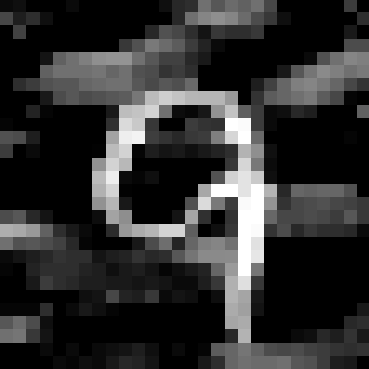
\includegraphics[width=0.2\textwidth]{Images/linf_s.png}
    \caption{Příklady vzorků vygenerovaných $l_\infty$ útokem} \label{linf_pic}
\end{figure}

Další komentář se bude věnovat obdobnnému problému, který vyvstal pro DSSIM útok
s parametrem velikosti výpočetního podokna $5$.
Podle Obrázku \ref{dssim_pic}
je okolí číslice silně znečištěno artefakty.
Kupodivu samotná číslice a její bezprostřední okolí je relativně nedotknuté.
Tento fenomén se vyskytl hlavně u volby velikosti výpočetního podokna $5$.
Vysvětlení zní jednoduše.
Neboť je původní benigní obrázek dál od číslice roven v každém pixelu nule,
pak SSIM index příslušných dvou podoken dál od číslice vychází konstantně skoro nula,
a to kvůli členu $\sigma_{x \tilde{x}}$ v čitateli.
Není úplně nula díky konstantě $C_2$, která zde vystupuje kvůli dělení.
Ta je ovšem dostatečně malá, aby byla převážena druhým členem gradientu.

\begin{figure}[h]
    \centering
    
\includegraphics[width=0.2\textwidth]{Images/dssim.png}
    \caption{Příklad vzorku vygenerovaného DSSIM útokem} \label{dssim_pic}
\end{figure}

\chapter{Robustnost neuronové sítě}

Předvedli jsme jev existence adversariálních vzorků
a z jeho vlastní povahy je zřejmé, že se jedná o nežádoucí jev.
Na tento fenomén potom odpovídá \emph{robustní strojové učení},
které se ve své podstatě snaží při učení neuronové sítě
danou neuronovou síť naučit tak, aby, pokud možno, k existenci adversariálních vzorků nedocházelo.
Obor robustního strojového učení potom nabízí řadu metod,
které k tomu mohou dopomoci.
Otázkou ale je, jak takovou metodu zařadit mezi ostatní ve smyslu jejího srovnání s ostatními metodami.
Potřebujeme proto ideálně číselné vyjádření toho,
jak si na tom daná neuronová síť, která byla učena daným algoritmem robustního strojového učení,
stojí ve smyslu náchylnosti na přítomnost jevu adversariálních vzorků.

\section{Přístup knihovny Foolbox}

Jednou z programovacích knihoven, která se snaží osvětlit tuto tématiku
a přinést nástroj pro výše nastíněné měření robustnosti modelu neuronové sítě,
je knihovna \emph{Foolbox} \cite{foolbox}.
Její přístup spočívá v implementaci pěti základních stavebních kamenů pro tvorbu
adversariálních vzorků.
Jsou to:
\begin{itemize}
    \item \emph{Model}, implementace rozhraní, které zajišťuje kompatibilitu knihovny s populárními
    knihovnami strojového učení (jako je i \emph{PyTorch});
    \item \emph{kritérium}, totiž pravidlo, podle kterého se rozhoduje, zda daný vzorek je adversariální
    či nikoliv;
    \item \emph{metrická vzdálenost}, to jest funkce, která vyjadřuje velikost perturbace
    potenciálního adversariálního vzorku (rozdíl $\tilde{x} - x$, užijeme-li zavedeného značení);
    \item \emph{algoritmus útoku}, způsob, jakým budou potenciální adversariální vzorky vyráběny;
    \item samotná \emph{adversariální perturbace}, což je výsledek algoritmu útoku.
\end{itemize}

Za komentář stojí, jaká že kritéria mohou být užita k určení adversariality vzorku.
S jedním jsme se již setkali v minulých kapitolách, totiž kritérium \emph{nesprávné klasifikace},
které spočívá ve vyhodnocení vzorku jako adversariálního právě při určení modelu,
že daný vzorek je v jiné třídě než původní vzorek, podle kterého je vzorek adversariální
tvořen.
Nemusíme zůstat pouze u tohoto kritéria.
Další kritéria lze odvodit při hlubším studiu pravděpodobnostního rozdělení, které model produkuje.
Takže např. kritérium \emph{top-k nesprávné klasifikace} spočívá v tom,
že vzorek je adversariální, pokud původní třída není mezi $k$~nejpravděpodobnějšími třídami.

Za zmíňku též stojí fakt, že knihovna Foolbox implementuje celou řadu různých adversariálních útoků.

\section{Přístup knihovny RobustBench}

Další programovací knihovnou, která se věnuje tématu robustnosti neuronových sítí
je knihovna \emph{RobustBench} \cite{robustbench}.
Tato knihovna jde o krok dál než knihovna Foolbox,
neboť její snahou je vyvinout jednotnotný test, který pro všechna nastavavení produkuje
jediné číslo, které lze tudíž hladce porovnat s ostatními výsledky.
Těchto testů je několik druhů, totiž pro datové sady \emph{CIFAR-10}, \emph{CIFAR-100} \cite{CIFAR}
a \emph{ImageNet} \cite{ImageNet}.
Následně podle zkoumané metriky jsou testy pro $l_\infty$ či $l_2$ útoky.
Výsledné číslo se potom nazývá \emph{robustní úspěšnost} (z angl. \emph{robust accuracy}),
jehož vyhodnocení spočívá ve vyčíslení průměrné úspěšnosti klasifikace poškozených vzorků
zkoumaným modelem v daném nastavení experimentu.
Tyto poškozené vzorky jsou postupně generovány procesem \emph{AutoAttack} \cite{AutoAttack},
který spočívá v postupném provádění čtyř typů adversariálních útoků.
Nejprve benigní vzorky projdou úpravou v podobě \emph{projected gradient descent} (\emph{PGD}) \cite{PGD}
s adaptivní velikostí kroku a ztrátou křížové entropie.
Dále vzorky, které zůstanou správně klasifikované projdou
obdobně procesem PGD, ale s jinou ztrátovou funkcí,
a to ztrátou rozdílu podílů hodnot funkce logit.
Poté je proveden \emph{cílený FAB útok} \cite{FAB},
následně \emph{black-box square attack} \cite{SquareAttack}.
Následně se výsledky agregují v již zmíněnou adversariální úspěšnost.
Tímm pádem lze metody robustního strojového učení mezi sebou porovnávat.


\chapter*{Závěr}

\pagestyle{plain}

\addcontentsline{toc}{chapter}{Záv\v{e}r}

V této práci bylo nastíněno téma problematiky adversariálních vzorků z jiného úhlu pohledu než bývá zvykem.
Cílem nebylo vyvinout novou metodu pro tvorbu adversariálních vzorků
ani najít, jak vhodně naučit model strojového učení tak, aby byl robustní vůči adversariálním útokům.
Cílem bylo nahlédnout na tuto problematiku z pohledu různorodosti metrik vizuální podobnosti
a poskytnout přehled, jak volba této metriky ovlivňuje tvorbu či podobu adversariálních vzorků.

Představili jsme tedy různé metriky vizuální podobnosti
a provedli jejich implementaci v programovacím jazyce \emph{Python} \cite{python}.
Dále jsme s pomocí knihovny \emph{PyTorch} \cite{pytorch} natrénovali jednoduchou neuronovou síť
pro klasifikaci číslic a tuto síť použili jako cíl námi implementovaného CW útoku
s možností volby užité metriky vizuální podobnosti.

Pro ovlivnění tvorby adversariálních vzorků se ukázal jako nežádoucí
iterativní charakter výpočtu aproximace Wassersteinovy vzdálenosti,
který nedovolil použít CW útok ke konstrukci adversariálních vzorků pomocí této metriky.
Další negativní dopad na tvorbu v podobě vysoké výpočetní náročnosti měla volba metriky založené na SSIM.

Ohledně samotné podoby vzorků vygenerovaných CW útokem lze říci,
že vzorky generované $l_\infty$ CW útokem byly velice poškozené,
jelikož derivace metriky indukované $l_\infty$ normou podle jedné z proměnných nezáleží na té dané proměnné,
leč na jednom jediném prvku.

S podobným problémem se bylo možné setkat při použití metriky vizuální podobnosti SSIM
s relativně malou velikostí podokna (vzhledem k celkové velikosti obrázku).
Takto vygenerované vzorky vykazovaly značně velkou přítomnost artefaktů v obrázku,
až na bezprostředně blízké okolí číslice.

Závěrem tedy lze říci, že na volbě metriky vizuální podobnosti záleží
a do budoucna lze tuto práci rozšířit jednak o další metriky vizuální podobnosti,
či o výsledky těch samých experimentů za použití jiné (bohatší) datové sady.


\begin{thebibliography}{1}
\addcontentsline{toc}{chapter}{Literatura}

\bibitem{advances}N. Akhtar, A. Mian, N. Kardan, M. Shah:
\emph{Advances in adversarial attacks and defenses in computer vision: A survey}.
IEEE Access 9, 2021, 155161-155196.

\bibitem{projected}W. Eric, F. Schmidt, Z. Kolter:
\emph{Wasserstein adversarial examples via projected sinkhorn iterations}.
International Conference on Machine Learning, PMLR, 2019.

\bibitem{foolbox}J. Rauber, R. Zimmermann, M. Bethge, W. Brendel:
\emph{Foolbox: A Python toolbox to benchmark the robustness of machine learning models}.
Reliable Machine Learning in the Wild Workshop, 34th International Conference on Machine Learning, 2017.

\bibitem{robustbench}F. Croce, M. Andriushchenko, V. Sehwag, E. Debenedetti, N. Flammarion, M. Chiang, P. Mittal, M. Hein:
\emph{RobustBench: a standardized adversarial robustness benchmark}.
Thirty-fifth Conference on Neural Information Processing Systems Datasets and Benchmarks Track (Round 2), 2021

\bibitem{vaserstejn} L. Vaserstein,
\emph{Markov processes over denumerable products of spaces, describing large systems of automata}.
Problemy Peredači Informacii 5, 1969.

\bibitem{ssim}Z. Wang, A. C. Bovik, H. R. Sheikh:
\emph{Image Quality Assessment: From Error Visibility to Structural Similarity}.
IEEE Transactions on Image Processing, ročník 13, č. 4, April 2004: s. 600–612.

\bibitem{wass_computation} M. Cuturi,
\emph{Sinkhorn Distances: Lightspeed Computation of Optimal Transport}.
Advances in Neural Information Processing Systems 26, 2013.

\bibitem{adv_opt} C. Szegedy, W. Zaremba, I. Sutskever, J. Bruna, D. Erhan, I. Goodfellow, R. Fergus,
\emph{Intriguing properties of neural networks}.
arXiv, 2014.

\bibitem{cw} N. Carlini, D. Wagner,
\emph{Towards evaluating the robustness of neural networks}.
IEEE Symposium on Security and Privacy (SP), IEEE, 2017.

\bibitem{MNIST} Y. Lecun, C. Cortes, C. J. Burges,
\emph{The mnist database of handwritten digits}. 1998.

\bibitem{RMSProp} G. Hinton,
\emph{Neural networks for machine learning}.
Coursera, video lectures, 2012.

\bibitem{CIFAR}A. Krizhevsky, G. Hinton:
\emph{Learning multiple layers of features from tiny images}.
Technical Report, 2009.

\bibitem{ImageNet}J. Deng, W. Dong, R. Socher, L.-J. Li, K. Li, L. Fei-Fei:
\emph{Imagenet: A large-scale hierarchical image database}.
IEEE conference on computer vision and pattern recognition, pages 248–255, Ieee, 2009.

\bibitem{AutoAttack}F. Croce, M. Hein:
\emph{Reliable evaluation of adversarial robustness with an ensemble of diverse parameter-free attacks}.
In ICML, 2020.

\bibitem{PGD} A. Mądry, A. Makelov, L. Schmidt, D. Tsipras, A. Vladu:
\emph{Towards deep learning models resistant to adversarial attacks}. Stat 1050 9, 2017.

\bibitem{FAB}F. Croce, M. Hein:
\emph{Minimally distorted adversarial examples with a fast adaptive boundary attack}.
ICML, 2020.

\bibitem{SquareAttack}M. Andriushchenko, F. Croce, N. Flammarion, M. Hein:
\emph{Square attack: a query-efficient black-box adversarial attack via random search}.
ECCV, 2020.

\bibitem{sinkhorn_thm}R. Sinkhorn:
\emph{A relationship between arbitrary positive matrices and doubly stochastic matrices}.
In The Annals of Mathematical Statistics 35, 876–879, 1964.

\bibitem{python}G. van Rossum:
\emph{Python tutorial, Technical Report CS-R9526}.
Centrum voor Wiskunde en Informatica (CWI), Amsterdam, 1995.

\bibitem{pytorch}A. Paszke, S. Gross, F. Massa, A. Lerer, J. Bradbury, G. Chanan, T. Killeen, Z. Lin, N. Gimelshein,
L. Antiga, A. Desmaison, A. Kopf, E. Yang,
Z. DeVito, M. Raison, A. Tejani, S. Chilamkurthy, B. Steiner, L. Fang, J. Bai, S. Chintala:
\emph{PyTorch: An Imperative Style, High-Performance Deep Learning Library}.
Advances in Neural Information Processing Systems 32, 8024–8035, 2019.

\end{thebibliography}

% \chapter*{Příloha}
% \addcontentsline{toc}{chapter}{Příloha}

% \lstinputlisting[language=Python, title=metrics.py]{../../code/metrics.py}

\end{document}
